\documentclass{journal}

\usepackage{graphicx}
\graphicspath{{../../drills}}


\usepackage{amsmath}
\usepackage[nopatch]{microtype}
\usepackage{booktabs}
\usepackage{hyperref}

\usepackage[left=2.45cm,top=3cm,right=2.45cm,bottom=2.5cm,bindingoffset=0cm]{geometry}

\title{Pocketing and Driving}

\author{}

\begin{document}
\maketitle
\noindent 

This session is about turning walls into pockets and driving out. 
Secondary focus on brace tracking.

\section*{Overview}

\subsection*{Off Skates Warm-up 5-10 Minutes Before the Session}
Lightly making sure that the joints still work.

Focus is {\bf not} on building strength, cardio or endurance, just on limbering up. Do 5 to 10 reps of each, on each side. 

\begin{itemize}
\item Toe taps + one leg light squats
\item Arm, shoulder and neck stretches
\item Opening and closing hip rotations
\item Knee raise to superman 
\item Cross chest knee raises
\item Butt kicks, high knees, side shuffles
\end{itemize}


\subsection*{Basic Warm-up - 15 minutes}

Mostly standard edge-work warm-up. Stage in faster laps rather than doing them all at once.
Do forwards and backwards.

\begin{itemize}
\item Sticky skating - Regular, Figure 8, low
\item Regular weaves + carves
\item One foot line-to-line (it not able, then \hyperref[drill:one_foot/serpentine]{serpentine}). 
\item One foot lateral 
\item Fast laps 
\item Stops
\end{itemize}





\subsection*{One Foot Blocking - 10 minutes}

Warming up edges with some contact. 
One skater driving, the other skater blocking on one foot. 
This will be a useful technique for resisting the driving drills to come.



\subsection*{Drives - 30 Minutes}
This next session is a revision on different driving drills.
Each drill should be run twice, once to feel out the movement, and the second time with a small modification.

\begin{itemize}
\item \hyperref[drill:drives/hip]{Hip drive} starting engaged
\item Hip drive from one to two feet 
\item \hyperref[drill:drives/shoulder]{Shoulder drive} 
\item \hyperref[drill:drives/low_shoulder]{Low shoulder drive}- with a focus on shoulder to butt cheek driving where possible. 
\item Shoulder drive into \hyperref[drill:drives/chest]{Chest drive}
\item \hyperref[drill:drives/shelf]{Shelf drive} starting engaged.
\end{itemize}

Blockers should attempt to resist, especially using the one foot blocking from earlier.
Blockers should act as if they were a butt in a wall - hence they cannot simply avoid the hit without displacing themselves 

The offence should be seeking to move the blocker at least one lane, but ideally to take them off the track. 


\subsection*{360 Offence - 10 minutes}

Mixing up the drives now, start with an offence engaged in a three wall. 

\begin{itemize}
\item Run the \hyperref[drill:three_wall/360_offence]{360 offence drill} - 30 seconds to 1 minute per offence, then a rest.
\item Move onto \hyperref[drill:three_wall/skewering]{skewering} practice.
\end{itemize}

This is a higher intensity drill, so cycling skaters for a rest is a good idea.



\subsection*{Two Wall Pocket and Drive - 15 minutes }
Jammer starts beind a colinear two wall. 
Butt is a filter, brace is a catch, butt then pockets. 
Brace catch can be a chest, a back or a sandbag.
\hyperref[drill:two_wall/double_lines]{Example figure here}.



\subsection*{Pocket and Drive - 30 minutes}
In three or two walls.
Jammer starts a foot behind, engaged blocker holds with back, disengaged blocker drives to a line for a pocket and hit out.


Optional cutting a friend.
Jammers are not allowed to be comfortable.


\subsection*{Four Walls - Remainder of the time}

Either a four wall \hyperref[drill:four_wall/pocket]{pocketing} drill or a four wall \hyperref[drill:four_wall/reset]{resetting} drill depending on the vibe.
See notes for the drill details.


\pagebreak


\section*{Drill Notes}


\input{../../drills/non_contact/one_foot/warm_up/serpentine}
\input{../../drills/non_contact/toe_stops/skating_to_toe_stop_movement}


\subsection*{Drill: 360 Offence}
\label{drill:three_wall/360_offence}

This drill requires four skaters, three blockers and an opposing offence. 


The original drill uses two to three different drives, I'll be updating this to four.

\begin{itemize}
    \item Hip drive using lateral pushes
    \item Shoulder to hip drive  
    \item Chest drive
    \item Shelf drive using lateral pushes 
\end{itemize}

The goal is to chain these drives together to dismember a wall.

The offence starts in the centre of the wall, where the jammer would normally be.

The offence should then attempt to drive one of the butts, switch and drive the brace then disengage and reset to drive the other butt towards the centre of the track before switching to again driving the brace. 
Then reset in the centre and repeat in the opposite direction.

Meanwhile the wall should seek to reform and counter the incoming offence.

% TODO: Fix link
%A video can be found \hyperref[https://www.youtube.com/watch?v=wZ6JcTYCBYw]{here}.

\begin{minipage}{0.48\textwidth}
\begin{center}

\includegraphics[scale=1,trim={0 1cm 0 4cm}, clip]{img/offence/360/1}


{\it Offence from within the seam, pushing out then taking the brace.}
\end{center}
\end{minipage}
\begin{minipage}{0.48\textwidth}
\begin{center}

\includegraphics[scale=1,trim={0 1cm 0 4cm}, clip]{img/offence/360/2}


{\it Offence starting from the line, optionally skewering, then taking the brace.} 
\end{center}
\end{minipage}



{\it Progressions}

As an offence progression - drive both butts together off the track as part of the final movement as in the skewering drill.

%As a natural progression, add a jammer.
% TODO: Figure

\subsection*{Drill: Double Lines}
\label{drill:two_wall/double_lines}

\begin{minipage}{0.38\textwidth}
\begin{centering}
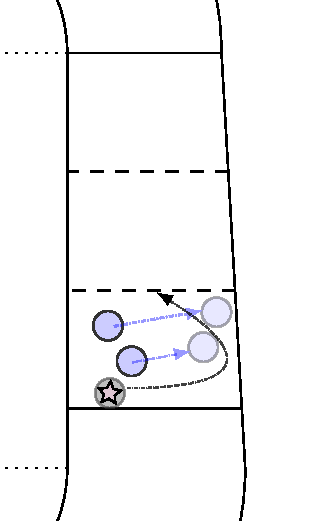
\includegraphics[scale=1.1,trim={0 0 0 4cm}, clip]{img/colinear_double_lines/escape}
{\it The approximate path of the jammer and blockers.}
\end{centering}

\end{minipage}
\hfill
\hspace{0.5cm}
\begin{minipage}{0.6\textwidth}


This drill involves a colinear two wall and a jammer.
There are four variations of this drill.

In rough order of difficult these are:
\begin{itemize}
\item Blocker in lane 1.5, brace in lane 1
\item Blocker in lane 3.5, brace in lane 4
\item Blocker in lane 1.5, brace in lane 2
\item Blocker in lane 3.5, brace in lane 3
\end{itemize} 


The jammer begins behind the rear blocker.

The goal of the jammer is to out-pace the wall to the other side of the track and pass the blockers in either lane 1 or lane 4.
The jammer must commit to this movement until they have passed the first blocker. 
\end{minipage}

\vspace{0.5cm}
\begin{minipage}{0.6\textwidth}

The goals of this drill vary depending on the level of the jammer and the blockers.

\begin{itemize}
\item The first goal is for the jammer to outpace the blockers sufficiently to escape.
\item The second is for the blockers to reach the line in time to prevent this. This will often involve the first blocker arriving too late, while the brace is in position to catch the jammer.
\item The third goal is for the jammer to avoid taking a double line and instead cut back into the seam.
\item Lastly, the blockers, after cutting off the line should close shoulders to prevent the jammer cutting through.
\end{itemize}
\end{minipage}
\hfill
\hspace{0.5cm}
\begin{minipage}{0.38\textwidth}
\begin{centering}
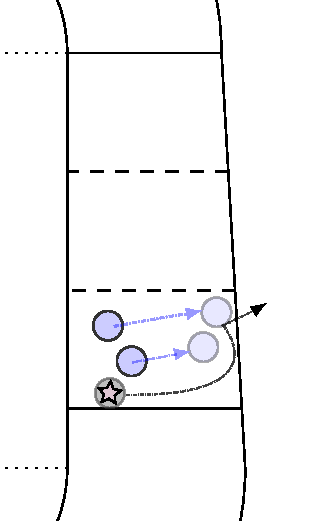
\includegraphics[scale=1.1,trim={0 0 0 4cm}, clip]{img/colinear_double_lines/caught}
{\it The jammer fails to cut back in and is caught or hit out.}
\end{centering}
\end{minipage}



% TODO Figure


\subsection{Four Wall Pocket}
\label{drill:four_wall/pocket}

This drill requires five skaters - four blockers, and a jammer. 

Starting in lane two or three, the jammer should be engaged with the wall. 
The fourth blocker should then approach the jammer from slightly behind and to the side, and using their chest drive the jammer out. The wall may rotate slightly to assist this, but the brace should remain on the line. 

The rest of the wall needs to remain rigid and strong - if the butts turn then the jammer will have purchase. 

The fourth blocker, while pushing, should establish a position where their rear leg is behind the jammer, cutting off that direction, while using their shoulders to rotate the jammer's shoulders out of the wall to face them.  
From this position the jammer has no legal movements as the blocker's backs are in the way, and the last blocker is preventing cutting back in. 
If the jammer holds position then they will be assessed a stop block, as a result the only legal action is to be knocked out of play. 


% TODO FIGURE

\subsection{Four Wall Reset}
\label{drill:four_wall/reset}

This drill requires six skaters - four blockers, a jammer and an offence.

Three blockers set up as a three wall, the fourth blocker should set up as an additional brace supporting both the three wall brace and one of the other blockers (typically the inside blocker).

The jammer should start engaged for this drill, while the offence is free to start either down or up track. 


The goal of this drill is for the fourth blocker to reform into the wall whenever the offence picks off a skater. The picked off blocker should then reform as the secondary brace.  
As some examples:

\begin{itemize}
    \item If the offence takes the brace, then the fourth blocker should take the brace position. 
    \item If the offence takes the blocker on the same side as the fourth blocker, then the blocker can sandbag, and slot back into that position. 
    \item Alternatively, if the opposite blocker is taken, then the brace can sandbag into that position, and the fourth blocker can replace the brace.
\end{itemize}

% TODO FIGURE











\end{document}
